\documentclass{sigchi}

% Load basic packages
\usepackage{balance}       % to better equalize the last page
\usepackage{graphics}      % for EPS, load graphicx instead
\usepackage[T1]{fontenc}   % for umlauts and other diaeresis
\usepackage{txfonts}
\usepackage{mathptmx}
\usepackage[pdflang={en-US},pdftex]{hyperref}
\usepackage{color}
\usepackage{booktabs}
\usepackage{textcomp}

% Some optional stuff you might like/need.
\usepackage{microtype}        % Improved Tracking and Kerning
% \usepackage[all]{hypcap}    % Fixes bug in hyperref caption linking
\usepackage{ccicons}          % Cite your images correctly!
% \usepackage[utf8]{inputenc} % for a UTF8 editor only

% Paper metadata (use plain text, for PDF inclusion and later
% re-using, if desired).  Use \emtpyauthor when submitting for review
% so you remain anonymous.
\def\plaintitle{Physical Effort and Expressivity in\\ Digital Musical Instruments}
\def\plainauthor{Tom Gurion}
\def\plainkeywords{Effort; Expression; Digital musical instruments.}

% llt: Define a global style for URLs, rather that the default one
\makeatletter
\def\url@leostyle{%
  \@ifundefined{selectfont}{
    \def\UrlFont{\sf}
  }{
    \def\UrlFont{\small\bf\ttfamily}
  }}
\makeatother
\urlstyle{leo}

% To make various LaTeX processors do the right thing with page size.
\def\pprw{8.5in}
\def\pprh{11in}
\special{papersize=\pprw,\pprh}
\setlength{\paperwidth}{\pprw}
\setlength{\paperheight}{\pprh}
\setlength{\pdfpagewidth}{\pprw}
\setlength{\pdfpageheight}{\pprh}

% Make sure hyperref comes last of your loaded packages, to give it a
% fighting chance of not being over-written, since its job is to
% redefine many LaTeX commands.
\definecolor{linkColor}{RGB}{6,125,233}
\hypersetup{%
  pdftitle={\plaintitle},
  pdfauthor={\plainauthor},
  pdfkeywords={\plainkeywords},
  pdfdisplaydoctitle=true, % For Accessibility
  bookmarksnumbered,
  pdfstartview={FitH},
  colorlinks,
  citecolor=black,
  filecolor=black,
  linkcolor=black,
  urlcolor=linkColor,
  breaklinks=true,
  hypertexnames=false
}

% create a shortcut to typeset table headings
% \newcommand\tabhead[1]{\small\textbf{#1}}

% End of preamble. Here it comes the document.
\begin{document}

\title{\plaintitle}

\numberofauthors{1}
\author{%
  \alignauthor{Tom Gurion\\
    \affaddr{Media and Arts Technology}\\
    \affaddr{Queen Mary University of London}\\
    \email{t.gurion@qmul.ac.uk}}\\
}

\maketitle

% TODO abstract
\begin{abstract}
  Lorem ipsum dolor sit amet, consectetur adipisicing elit, sed do eiusmod tempor incididunt ut labore et dolore magna aliqua. Ut enim ad minim veniam, quis nostrud exercitation ullamco laboris nisi ut aliquip ex ea commodo consequat. Duis aute irure dolor in reprehenderit in voluptate velit esse cillum dolore eu fugiat nulla pariatur. Excepteur sint occaecat cupidatat non proident, sunt in culpa qui officia deserunt mollit anim id est laborum.
\end{abstract}

\keywords{\plainkeywords}

\section{Introduction}

The use of computers and digital instruments is common in nowadays musical performances.
TODO one more sentence here.
One significant difference between traditional and digital musical instruments performances is that physical effort is usually involve in the former, but can be totally absent in the later.
This difference presents several issues, most of these thorouly explored in the context of laptop music.

TODO paragraph explaining laptop music.

For example, a common criticism is that the audiance might fail to understand the performance.
On the extreme, a listener might question the "liveness" of a performance altogether when unable to tell the difference between live and pre-composed playback.
Besides, visible effort is an important expressive tool in many musical contexts.
TODO BETTER EXAMPLES
Consider, for example, a trumpet player and his outcurved veins in the neck while he reaches a high note, or a drummer, sweating during intense performance.

TODO Define the issue better. Digital musical instruments are not laptop music, but some of the issues overlap.

Theoretical studies from the last few decades highlited these issues.
Some researchers explain the core of the problem by the lack of apparant relationship between the way an instrument is played and the resulted sound \cite{Schloss2003,DEscrivan2006}.
Others argue that computers promote "effortless interaction" and by that contradict they way music should be created \cite{Ryan1992}.
Most of the research in the field, however, doesn't confront the theoretical hypotheses using rigrous experiments.
One exception is a recent experiment based study by Bown et al.\ \cite{Bown2014}.
Their results show that listeners do able to perceive what the performer is doing from the audio alone.

Along with these lines, the current study examines to what extent physical effort can enhance expressivity in playing digital instruments.
In addition, it explores the effect of the performer's physical effort on the audience perception and appreciation of the performance.
These questions are assessed in controlled experiment, evaluating perceived expressivity from the point of view of the performer and the listener alike.

The current work uses the Schleikess interface, a digital controller for interactive performance that requires physical effort and large body movements from the performer, to assess performance expressivity.
Figure \ref{fig:schleikess} shows a schematic diagram of the interface.
It is composed of two elastic bands, each of them is connected with one side, through a load sensor, to the belt loop of the performer.
The performer holds the other side of the elasic bands and can strech them to play.

This controller can be used for different creative purposes.
In the context of this study one elastic band controls the pitch and the other controls the amplitude of a sawtooth tone generator.
TODO discuss more this type of interaction. Simple relationship between gestures and produced sound helps the audience to understand the performance. TODO search and reference the theramin design decition.

\begin{figure}
  \centering
  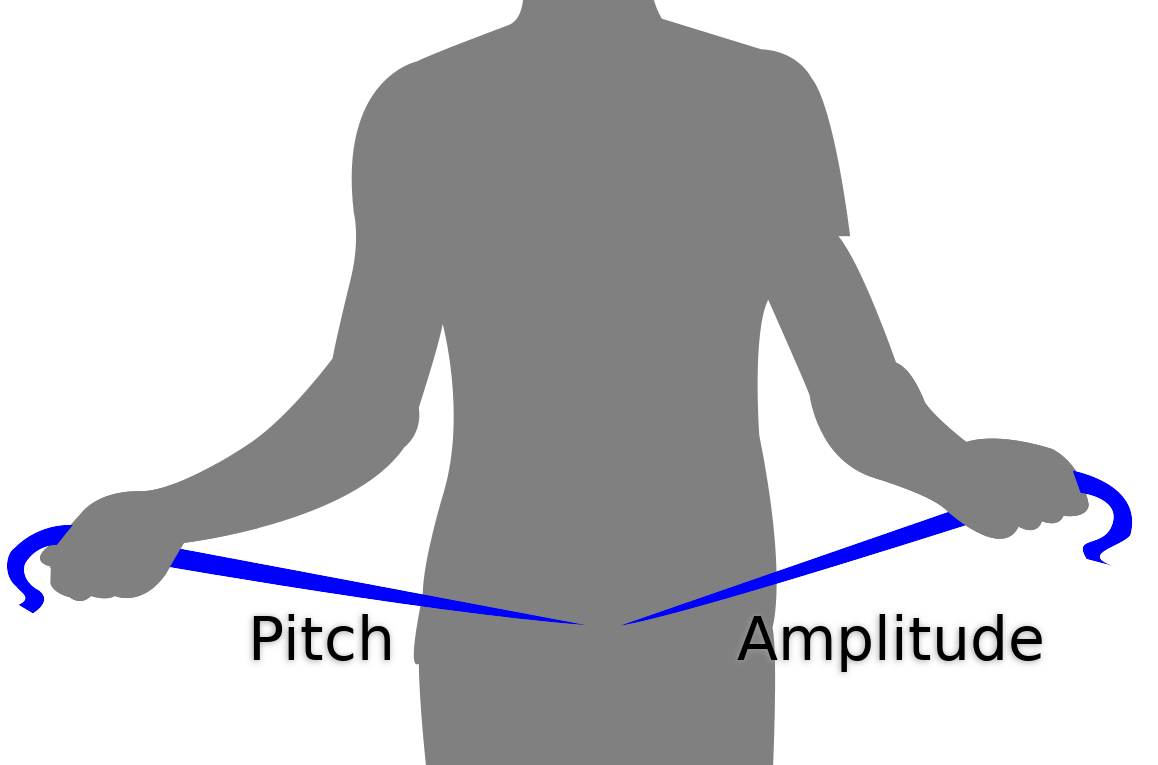
\includegraphics[width=0.9\columnwidth]{figures/schleikess}
  \caption{A diagram of the Schleikess interface. In blue are the two elastic bands. Stretching the left raises the pitch and stretching the right raises the amplitude.}~\label{fig:schleikess}
\end{figure}

\section{Initial study}

\subsection{Methods}

\begin{figure}
  \centering
  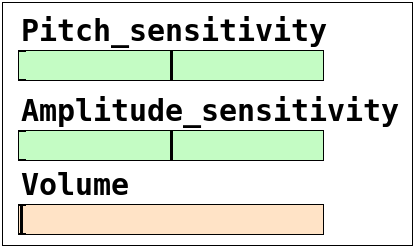
\includegraphics[width=0.9\columnwidth]{figures/pd_interface}
  \caption{The Schleikess graphical interface. Three sliders controll the sensitivity of the pitch band to force, the sensitivity of the amplitude band to force, and the overall volume of the instrument.}~\label{fig:pd-interface}
\end{figure}

In this initial study I examined to what extent physical effort can enhance expressivity in playing digital instruments.
TODO more specifically... Controllability, range of possibilities. Or maybe just in the discussion.

TODO X participants were invited to play with the Schleikess based synthesiser and discuss their subjective experience.
Apart from the physical interface, figure \ref{fig:pd-interface} shows the interface on the computer screen that was exposed to the participants.
The interface presents three sliders.
The first two controll the sensitivity of each elastic band to force.
So, when the sensitivity is set to low value, a major physical force is needed to raise the pitch or amplitude, but when the sensitivity is set to high value even minor changes affect the output significantly.
The last slider controlls the overall volume of the instrument and allows the participant to set it to a comfortable hearing level.

First, I explained to the participants that stretching the elastic bands controlls the instrument.
The relationship between stretching the bands and the resulted sound was not explaind.
Than, the participants were asked to play the instrument until they understand the mapping between gestures and sound.
During this time they could also set the volume to a comfortable hearing level.
After familiarize themselves with the instrument they were asked to set the sensitivity sliders to the values they like the most.
Later, I discussed the experience of playing the instrument with each participant.
The discussion concentrated around the question of why they choose these particular sensitivity settings.
In some of the discussions the participants referred to how expressive and controllable the instrument felt.
In these cases I asked them to elaborate and explain the terms, and why they felt this way.
However, participants that didn't mentioned these concepts in the first place were not forced to talk about them.

This type of exploratory initial study is designed to get basic insights about the relationships between physical effort and expressivity.
Provided that there is almost no empirical research in this field, this type of broad exploration is necessary to gain first insights, and to be able to design a more thorough experiment, as I will describe later.

\subsection{Results}

Most of the participants in the study, TODO out of TODO, understood how the instrument works by trying it out.
I explained the relationship between pulling the elasic bands and the resulted sound to those who find it hard to understand.
After the explaination they continued with the experiment like the rest of the participants.

TODO participants explicitly discussed the balance between having range of possibilities and controllability with relationship to the sensitivity of the instrument to force.
This was significantly apparant in the discussion of the pitch sensitivity.
TODO participants wanted to maximize the pitch range that the instrument produces by raising the sensitivity, but no participant set the pitch sensitivity to the maximum value.
TODO participants explicitly explained that they kept the pitch sensitivity below the maximum value to make sure they can control the instrument.
On the other hand, only TODO participants kept the pitch sensitivity low, and explained this preference by not liking notes with high pitch in general.

Most of the participants presented different explanations for choosing the sensitivity values for the pitch and for the amplitude.
Only TODO of the participants used the same reasoning for setting the two sliders.

TODO participants mentioned that playing the instrument felt like a physical exercise, is somewhat tedious, or made them pain over time.
Therefore, TODO prefered to minimize effort or movement while playing.
One participant, attempting to minimize the effort involve in large hand movement, described a completely different playing technique.
Instead of pull and release the bands, the participant held them in constant force and change the tention by pushing the pinky against the bands.

\section{Discussion}

Lorem ipsum dolor sit amet, consectetur adipisicing elit, sed do eiusmod tempor incididunt ut labore et dolore magna aliqua. Ut enim ad minim veniam, quis nostrud exercitation ullamco laboris nisi ut aliquip ex ea commodo consequat. Duis aute irure dolor in reprehenderit in voluptate velit esse cillum dolore eu fugiat nulla pariatur. Excepteur sint occaecat cupidatat non proident, sunt in culpa qui officia deserunt mollit anim id est laborum.

\subsection{Future research}

Lorem ipsum dolor sit amet, consectetur adipisicing elit, sed do eiusmod tempor incididunt ut labore et dolore magna aliqua. Ut enim ad minim veniam, quis nostrud exercitation ullamco laboris nisi ut aliquip ex ea commodo consequat. Duis aute irure dolor in reprehenderit in voluptate velit esse cillum dolore eu fugiat nulla pariatur. Excepteur sint occaecat cupidatat non proident, sunt in culpa qui officia deserunt mollit anim id est laborum.

% BALANCE COLUMNS
\balance{}

% REFERENCES FORMAT
% References must be the same font size as other body text.
\bibliographystyle{SIGCHI-Reference-Format}
\bibliography{bib}

\end{document}

%%% Local Variables:
%%% mode: latex
%%% TeX-master: t
%%% End:
